\documentclass{article}
\usepackage{graphicx} % Required for inserting images
\usepackage{geometry}
\usepackage{circuitikz}
\usepackage{siunitx}
\usepackage{CJKutf8}
\usepackage{amsmath}
\usepackage{amssymb}
\usepackage{caption}
\usepackage{float}
\usepackage{subcaption}
\geometry{top=5mm, left=30mm, a4paper}

\title{Common-Source Amplifier Analysis Report}
\author{梁程捷 (B11901136), 吳奕娃 (B11901080)}
\date{}


\begin{document}
\begin{CJK*}{UTF8}{bkai}

\maketitle

\section*{DC analysis}
\begin{table}[H]
    \begin{center}
    \begin{tabular}{|c|c|c||c|c|c|}
        \hline
        $V_G$ (V)& $V_D$ (V) & $V_S$ (V)& $I_G$ (\unit{\milli\ampere}) & $I_D$ (\unit{\milli\ampere})& $I_S$ (\unit{\milli\ampere})\\ 
        \hline\hline
        7.285   & 5.497 & 9.857 & 0.001 & 0.548 & 0.549 \\

     \hline
    \end{tabular}
    \caption{DC analysis raw experimental data}
    \end{center}
\end{table}

\section*{Small-signal analysis}
\textbf{Frequency of input waveform $ f = 10$ \unit{\kilo\hertz}}\\
\begin{table}[H]
    \begin{center}
    \begin{tabular}{|c|c|c|c|}
        \hline
            & CH1 (V) & CH2 (V) & CH2 / CH1\\ 
        \hline\hline
        $\left\lvert v_o/v_{sig} \right\rvert$  with $C_s$ & 0.456 & 4.16 & 9.12     \\
        $\left\lvert v_o/v_{i} \right\rvert$  with $C_s$ & 0.432 & 5.84 & 13.5     \\
        $\left\lvert v_o/v_{sig} \right\rvert$  without $C_s$ &0.448 & 0.220 & 0.491   \\
        $\left\lvert v_o/v_{i} \right\rvert$  without $C_s$ &0.456 & 0.268 & 0.588   \\

     \hline
    \end{tabular}
    \caption{Small-signal analysis raw experimental data}
    \end{center}
\end{table}

\subsection*{waveforms}
\begin{figure}[h]
    \begin{center}
    
        \begin{subfigure}[b]{0.35\textwidth}
            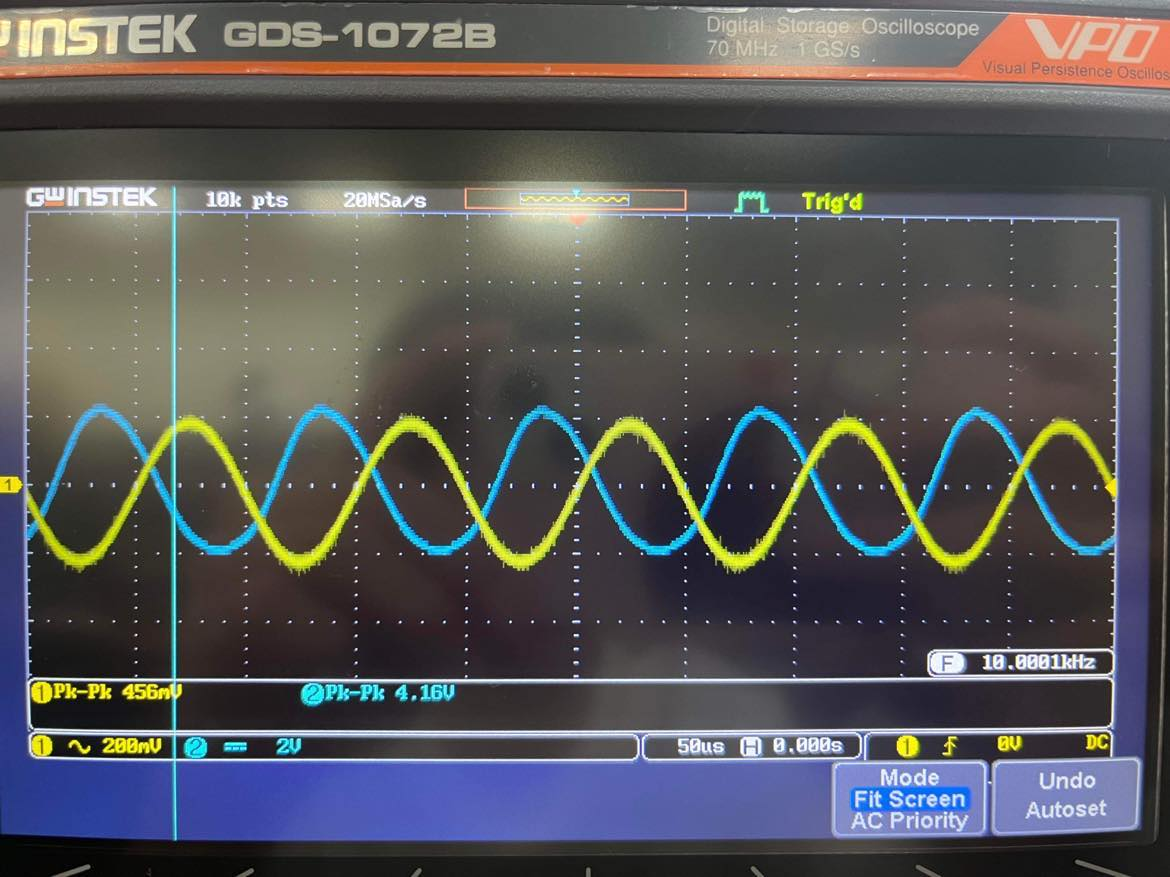
\includegraphics[width=\textwidth]{vsig_cs.jpg}
            \caption{$\left\lvert v_o/v_{sig} \right\rvert$ with $C_s$}
        \end{subfigure}
        ~
        \begin{subfigure}[b]{0.35\textwidth}
            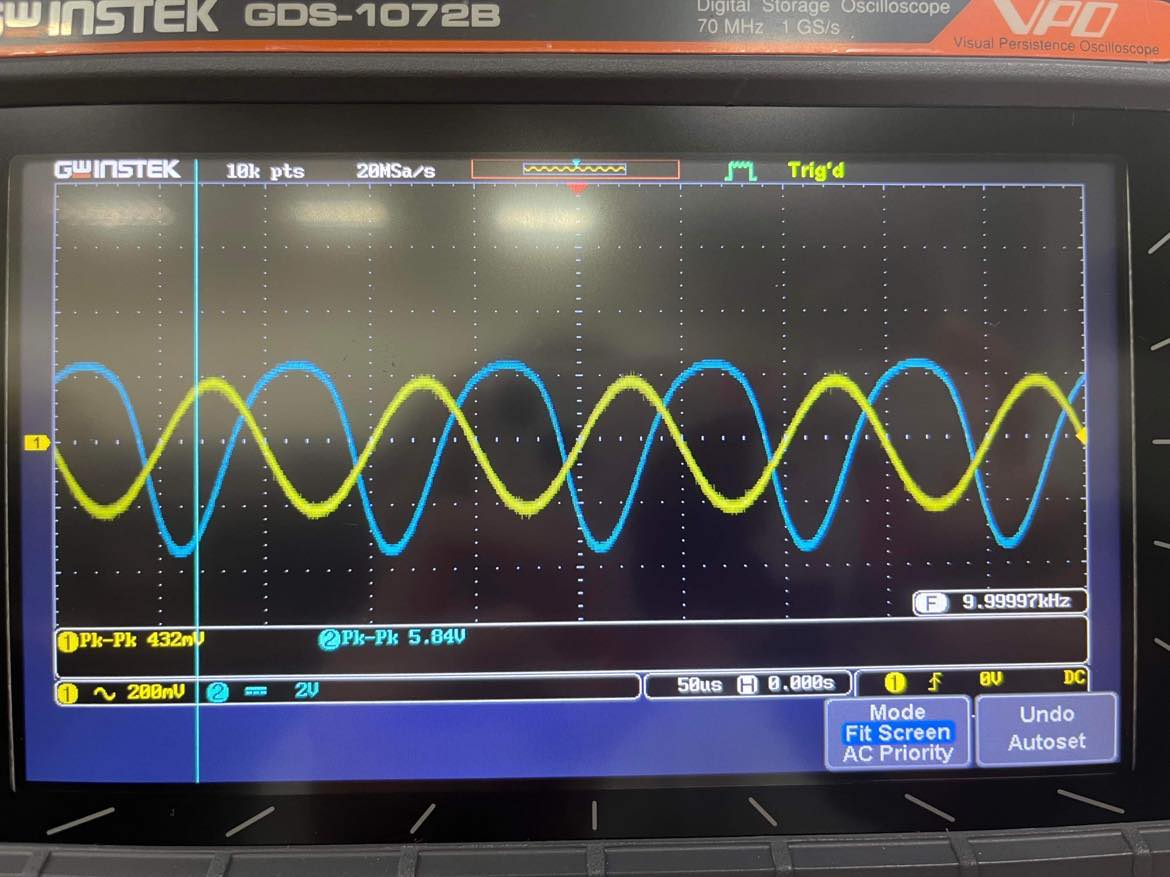
\includegraphics[width=\textwidth]{vi_cs.jpg}
            \caption{$\left\lvert v_o/v_{i} \right\rvert$ with $C_s$}
        \end{subfigure}

        \begin{subfigure}[b]{0.35\textwidth}
            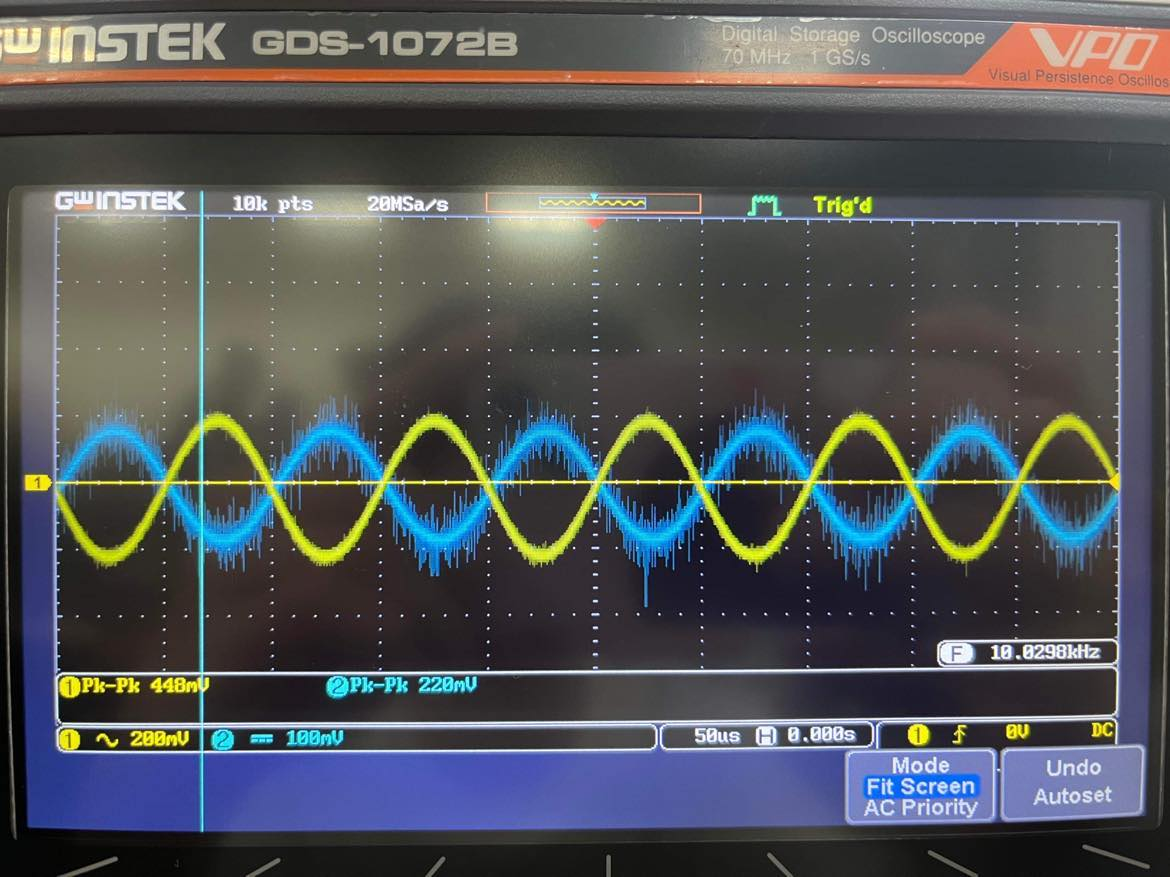
\includegraphics[width=\textwidth]{vsig_wcs.jpg}
            \caption{$\left\lvert v_o/v_{sig} \right\rvert$ without $C_s$}
        \end{subfigure}
        ~
        \begin{subfigure}[b]{0.35\textwidth}
            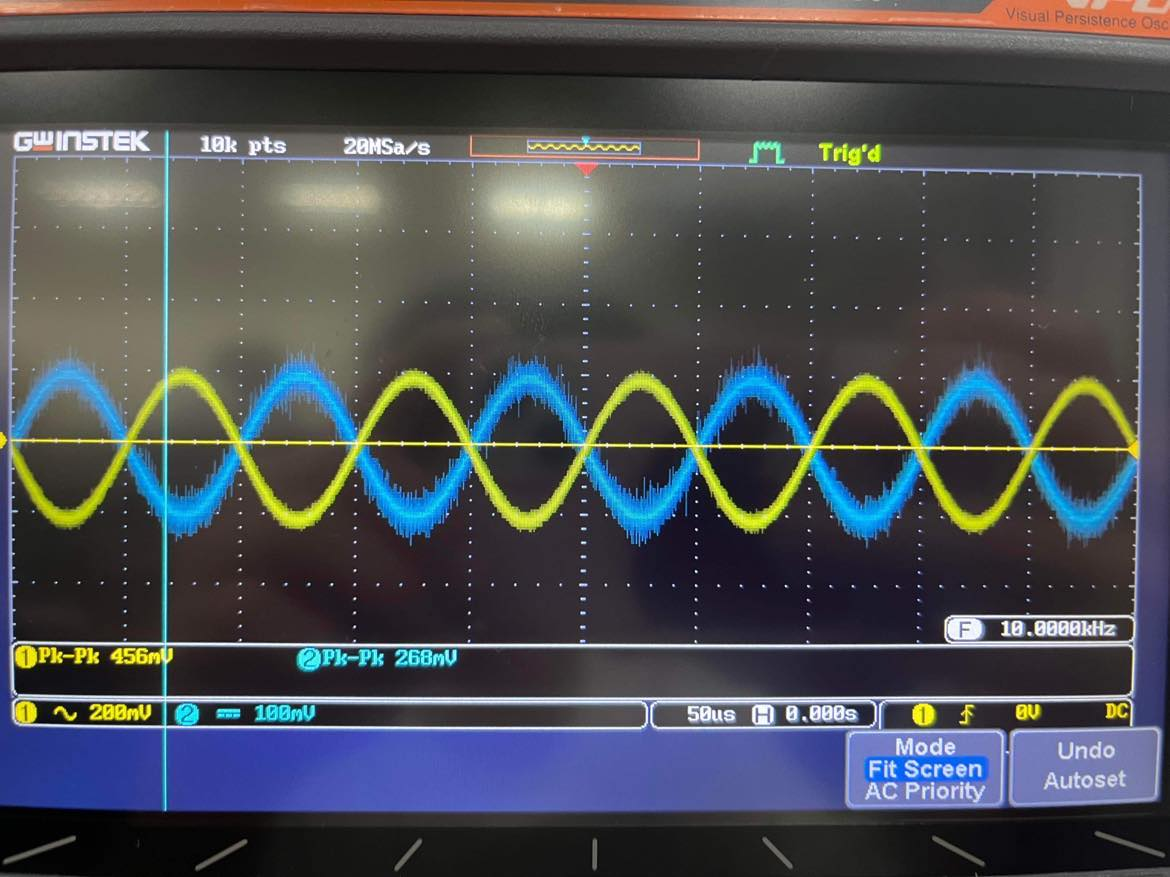
\includegraphics[width=\textwidth]{vi_wcs.jpg}
            \caption{$\left\lvert v_o/v_{i} \right\rvert$ without $C_s$}
        \end{subfigure}
    \end{center}
\end{figure}
\textbf{Conclusion: The gain without bypass capacitor (degenerate) is much lower than the one with bypass capacitor, which is concurrent with theoretical expectation.}

\end{CJK*}
\end{document}

